
%% Based on a TeXnicCenter-Template by Tino Weinkauf.
%%%%%%%%%%%%%%%%%%%%%%%%%%%%%%%%%%%%%%%%%%%%%%%%%%%%%%%%%%%%%

%%%%%%%%%%%%%%%%%%%%%%%%%%%%%%%%%%%%%%%%%%%%%%%%%%%%%%%%%%%%%
%% HEADER
%%%%%%%%%%%%%%%%%%%%%%%%%%%%%%%%%%%%%%%%%%%%%%%%%%%%%%%%%%%%%
%\documentclass[onecolumn, 11pt, conference, compsocconf]{IEEEtran}
\documentclass[onecolumn, 12pt, article]{IEEEtran}
\usepackage{times,color,amsmath,amssymb,amsthm,comment,graphicx,cite,multirow}
%\documentclass[letterpaper,oneside,11pt]{letter}
% Alternative Options:
%	Paper Size: a4paper / a5paper / b5paper / letterpaper / legalpaper / executivepaper
% Duplex: oneside / twoside
% Base Font Size: 10pt / 11pt / 12pt


%% Language %%%%%%%%%%%%%%%%%%%%%%%%%%%%%%%%%%%%%%%%%%%%%%%%%
\usepackage[USenglish]{babel} %francais, polish, spanish, ...
\usepackage[T1]{fontenc}
\usepackage[ansinew]{inputenc}

\usepackage{lmodern} %Type1-font for non-english texts and characters
\usepackage{algorithm}
\usepackage{algpseudocode}
\usepackage{float}

%% Packages for Graphics & Figures %%%%%%%%%%%%%%%%%%%%%%%%%%
%\usepackage{graphicx} %%For loading graphic files
%\usepackage{subfig} %%Subfigures inside a figure
%\usepackage{tikz} %%Generate vector graphics from within LaTeX

%% Please note:
%% Images can be included using \includegraphics{filename}
%% resp. using the dialog in the Insert menu.
%% 
%% The mode "LaTeX => PDF" allows the following formats:
%%   .jpg  .png  .pdf  .mps
%% 
%% The modes "LaTeX => DVI", "LaTeX => PS" und "LaTeX => PS => PDF"
%% allow the following formats:
%%   .eps  .ps  .bmp  .pict  .pntg


%% Math Packages %%%%%%%%%%%%%%%%%%%%%%%%%%%%%%%%%%%%%%%%%%%%
\usepackage{amsmath}
\usepackage{amsthm}
\usepackage{amsfonts}
\usepackage{amssymb}
%\usepackage{array,MnSymbol}


%% Line Spacing %%%%%%%%%%%%%%%%%%%%%%%%%%%%%%%%%%%%%%%%%%%%%
\usepackage{setspace}
\singlespacing        %% 1-spacing (default)
%\onehalfspacing       %% 1,5-spacing
%\doublespacing        %% 2-spacing


%% Other Packages %%%%%%%%%%%%%%%%%%%%%%%%%%%%%%%%%%%%%%%%%%%
%\usepackage{a4wide} %%Smaller margins = more text per page.
\usepackage{fancyhdr} %%Fancy headings
\usepackage{listings}
\usepackage{capt-of}


%
% Theorem like environments
%
\newtheorem{problem}{Problem}%
%\numberwithin{problem}{section}
\newtheorem{theorem}{Theorem}%
\newtheorem{acknowledgment}{Acknowledgment}%
%\newtheorem{algorithm}{Algorithm}%
\newtheorem{assumption}{Assumption}%
\newtheorem{axiom}{Axiom}%
\newtheorem{case}{Case}%
\numberwithin{case}{problem}
\newtheorem{claim}{Claim}%
\newtheorem{conclusion}{Conclusion}
\newtheorem{condition}{Condition}
\numberwithin{condition}{problem}
\numberwithin{condition}{subsection}
\newtheorem{conjecture}{Conjecture}
\newtheorem{corollary}{Corollary}
\newtheorem{criterion}{Criterion}
\newtheorem{definition}{Definition}
\numberwithin{definition}{section}
\newtheorem{example}{Example}
\newtheorem{exercise}{Exercise}%
\newtheorem{lemma}{Lemma}%
\newtheorem{notation}{Notation}%
\theoremstyle{remark}
\newtheorem{question}{Question}%
\numberwithin{question}{problem}
\theoremstyle{plain}
\newtheorem{answer}{Answer}%
\numberwithin{answer}{problem}
\newtheorem{proposition}{Proposition}%
\newtheorem{remark}{Remark}%
\newtheorem{solution}{Solution}%
\numberwithin{solution}{section}
\newtheorem{summary}{Summary}%
\numberwithin{equation}{section}%
\newtheorem{option}{Option}



\raggedbottom
%%%%%%%%%%%%%%%%%%%%%%%%%%%%%%%%%%%%%%%%%%%%%%%%%%%%%%%%%%%%%
%% Remarks
%%%%%%%%%%%%%%%%%%%%%%%%%%%%%%%%%%%%%%%%%%%%%%%%%%%%%%%%%%%%%
%
% Note:
% 1. Edit the used packages and their options (see above).
% 2. If you want, add a BibTeX-File to the project
%    (e.g., 'literature.bib').
% 3. Happy TeXing!
%
%%%%%%%%%%%%%%%%%%%%%%%%%%%%%%%%%%%%%%%%%%%%%%%%%%%%%%%%%%%%%

%%%%%%%%%%%%%%%%%%%%%%%%%%%%%%%%%%%%%%%%%%%%%%%%%%%%%%%%%%%%%
%% Options / Modifications
%%%%%%%%%%%%%%%%%%%%%%%%%%%%%%%%%%%%%%%%%%%%%%%%%%%%%%%%%%%%%

%\input{options} %You need a file 'options.tex' for this
%% ==> TeXnicCenter supplies some possible option files
%% ==> with its-templates (File | New from Template...).




%% BEGIN DOCUMENT
\begin{document}

%% Title Page
\title{0/1 Knapsack}
\author{Preston Stosur-Bassett}
\date{March 11, 2015}
\maketitle

\pagestyle{fancy}
\fancyhead[R]{0/1 Knapsack in Java, page \thepage}
\fancyhead[L]{Preston Stosur-Bassett}

%% BEGIN ABSTRACT
\begin{abstract}
%%TODO: write this

%% END ABSTRACT
\end{abstract}

%% BEGIN MOTIVATION
\section{Motivation}
A 0/1 Knapsack problem is most often described as how does a theif steal the most valuable items with the amount of space he has available to carry them. However, the applications of a 0/1 Knapsack far beyond just this. When solved, a 0/1 Knapsack problem will render the optimal solution, whether it be how one should construct their schedule so they can get the most done in one day, or how to pack a truck such that the fewest amount of trips are taken. 

%% END MOTIVATION

%% BEGIN BACKGROUND
\section{Background}
Unfortunately, solving a 0/1 Knapsack problem often times proves difficult because in order to find the best solution, all possible solutions must be attempted, a method known as brute force. It is not pratical to brute force a problem of this kind because it would take $ \theta{n!} $ to solve, which is unacceptable for large sets of numbers. However, there are other methods beside brute force that allow for the correct or 'good-enought' solution to be found. One of these methods is known as dynamic programming, which trades off speed for space. With dynamic programming the correct solution can be found in $ \theta{n*m} $ time, where n is the amount of items and m is the size of the knapsack. Another method for solving this type of problem is called a greedy algorithm, which works by making the best decision on which item to take locally. A greedy solution to the 0/1 Knapsack problem traditionally runs in $ \theta{n} $ time. Unfortunately a greedy solution is not always correct and therefore highly unreliable.

%% END BACKGROUND

%% BEGIN PROCEDURE
\section{Procedure}
A multidimentional array insertion sort can be implemented in a multitude of languages using the pseudocode provided in Algorithm 1.
\newline
\textbf{Insertion Sort Pre-Condition}: A is an unsorted non-empty array of non-empty arrays containing a comparable data type with a natural order such that v is an index value of the inner array.
\newline
\textbf{Insertion Sort Post-Condition}: A' is a permutation of A that is in strictly non-increasing order.
\begin{algorithm}
\caption {\textsc{Insertion-Sort}(A, v)}
\label{algo:insertionsort}
\begin{algorithmic}[1]
\Procedure{Insertion-Sort}{A, v}
\If{$A.length < 2$}
\State{\Return{$A$}}
\EndIf
\State{$i = 2$}
\While{$i$ upto $A.length$}
	\State{$key = A[i][v]$}
	\State{$a = A[i]$}
	\State{$j = i - 2$}
	\While{$j$ downto $1$ and $key > A[j][v]$}
		\State{$A[j+1] = A[j]$}
		\State{$j = j - 1$}
	\EndWhile
	\State{$A[j+1] = a$}
	\State{$i = i + 1$}
\EndWhile
\State{\Return{$A$}}
\EndProcedure
\end{algorithmic}
\end{algorithm}
\newline
\textbf{Insertion Sort Outer-Loop Invariant}: The subarray A'[1 ... i - 1] contains all the same elements as the subarray A[1 ... i - 1].
\newline 
\textbf{Insertion Sort Outer-Loop Initialization}: The outer-loop invariant holds because A'[1 ... i - 1] and A[1 ... i - 1] both contain the same one element.
\newline
\textbf{Insertion Sort Outer-Loop Maintenance}: The outer-loop invariant holds because A'[1 ... i - 1] and A[1 ... i - 1] both contain the same elements, although they may be in different orders.
\newline
\textbf{Insertion Sort Outer-Loop Termination}: When the outer-loop terminates, i = A.length, which implies that the entire array has been traversed and the guard has been negated. The negation of the guard implies that A'[1 ... i - 1] contains all the elements in A[1 ... i - 1].
\newline
\newline
\textbf{Insertion Sort Inner-Loop Invariant}: A'[1 ... j] is sorted in strictly non-decreasing order.
\newline
\textbf{Insertion Sort Inner-Loop Initialization}: Before the first iteration of the loop, j = 1, meaning the subarray A'[1 ... j] contains exactly one element, which is already sorted.
\newline
\textbf{Insertion Sort Inner-Loop Maintenance}: At the beginning of each iteration of the loop the inner-loop invariant holds because j counts down from i, and A'[j+1] is swapped with A'[j] only if A'[j+1] is less than A[j].
\newline
\textbf{Insertion Sort Inner-Loop Termination}: The negation of the guard implies that j = A.length and that A'[1 ... j] has been entirely traversed and sorted in strictly non-decreasing order, which maintains the inner-loop invariant. 
\newline
\newline
\textbf{Insertion Sort Conclusion}: The termination of both the inner and outer loops implies that the entire array has been traversed, A' is a permutation of A containing all the same elements in strictly non-decreasing order. This satisfies the post condition.
\newline
\newline

A greedy solution to a 0/1 knapsack problem can be implemented in a variety of languages using the pseudocode in Algorithm 2.
\newline
\textbf{Greedy Knapsack Pre-Condition}: $Weights$ and $Prices$ both have in them $n$ number of elements
\newline
\textbf{Greedy Knapsack Post-Condition}: The returned value will be a reasonable solution for the largest value of price combinations such that the aggregate of the corresponding weights does not exceed knapsack capacity $c$.
\begin{algorithm}
\caption {\textsc{Greedy-Knapsack}(n, Weights, Prices, c)}
\label{algo:greedy}
\begin{algorithmic}[1]
\Procedure{Greedy-Knapsack}{n, Weights, Prices, c}
\If{$n == 1$ and $Weights[1] <= c$}
	\State{\Return{$Prices[1]$}}
\EndIf
\If{$n <= 0$}
	\State{\Return{$0$}}
\EndIf
\State{$profit = 0$}
\State{$ratio = new Array$}
\For{$v = 1$ upto $n$}
	\State{$a = Prices[v] / Weights[v]$}
	\State{$ratio[v] = a$}
\EndFor
\State{$ratio = Insertion-Sort(ratio, 1)$}
\State{$i = 1$}
\While{$c > 0$ and $i < n$}
	\If{$c - ratio[i][3] >= 0$}
		\State{$profit = profit + ratio[i][2]$}
		\State{$c = c - ratio[i][3]$}
	\EndIf
	\State{$i = i + 1$}
\EndWhile
\State{\Return{$profit$}}
\EndProcedure
\end{algorithmic}
\end{algorithm}
\newline
\textbf{Greedy Solution First-Loop Invariant}: ratio[1 ... v-1] has the same number of non-null elements in it as both Prices[1 ... v-1] and Weights[1 ... v-1].
\newline
\textbf{Greedy Solution First-Loop Invariant Initialization}: The invariant holds true before the first iteration of the loop because $v=1$, and ratio[1 ... v-1], Prices[1 ... v-1] and Weights[0 ... v-1] all do not exist, and is therefore vacuously true.
\newline
\textbf{Greedy Solution First-Loop Invariant Maintenance}: At the beginning of each iteration of the loop the invariant holds true because each time the loop runs, v is incremented by 1, and exactly 1 element is added to ratio, therefore ratio[0 ... v-1] will have the exact same number of elements as both Prices[1 ... v-1] and Weights[1 ... v-1].
\newline
\textbf{Greedy Solution First-Loop Invariant Termination}: After the termination of the loop the invariant holds true because v has been incremented by 1 during each iteration of the loop, and ratio has gained 1 element during each iteration of the loop, therefore ratio[1 ... v-1] contains the exact same number of elements as both Prices[1 ... v-1] and Weights[1 ... v-1].
\newline
\newline
\textbf{Greedy Solution Second-Loop Invaraint}: The aggregate of the weights corresponding to the prices included in $profit$ are less than or equal to $c$.
\newline
\textbf{Greedy Solution Second-Loop Invariant Initialization}: Before the first iteration of the loop the invariant holds true vacuously because no prices have been included in $profit$.
\newline
\textbf{Greedy Solution Second-Loop Invariant Maintenance}: At the beginning of each iteration of the loop the invariant holds true because only items whose weight is less than or equal to the size of $c$ are added to $profit$.
\newline
\textbf{Greedy Solution Second-Loop Invariant Termination}: After the termination of the loop, the invariant holds true because only items whose weight was less than or equal to the value of $c$ have been added to $profit$.
\newline
\newline

A dynamic solution to 0/1 knapsack can be implemented in a variety of languages using the pseudocode provided in Algorithm 3.
\newline
\textbf{Dynamic Knapsack Pre-Condition}: $Weights$ and $Prices$ both have $n$ number of elements
\newline
\textbf{Dynamic Knapsack Post-Condition}: The returned value will be the correct solution for the largest value of price combinations such that the aggregate of the corresponding weights does not exceed knapsack capacity $c$.
\begin{algorithm}
\caption {\textsc{Dynamic-Knapsack}(n, Weights, Prices, c)}
\label{algo:dynamic}
\begin{algorithmic}[1]
\Procedure{Dynamic-Knapsack}{n, Weights, Prices, c}
\If{$n == 1$ and $Weights[1] <= c$}
	\State{\Return{$Prices[1]$}}
\EndIf
\If{$n <= 0$}
	\State{\Return{$0$}}
\EndIf
\State{$tab[n][c] = new Nested Array$}
\For{$x = 1$ upto $n$}
	\For{$y = 1$ upto $c$}
		\State{$tab[x][y] = 0$}
	\EndFor
\EndFor
\For{$i = 1$ upto $n$}
	\For{$j = 0$ upto $c$}
		\If{$Weights[i] <= j$ and $Prices[i] + tab[i][j - Weights[i]] > tab[i][j]$}
			\State{$tab[i+1][j] = Price[i] + tab[i][j - weights[i]]$}
		\EndIf
		\If{$!$$(Weights[i] <= j)$ and $!$$(Prices[i] + tab[i][j - Weights[i]] > tab[i][j])$}
			\State{$tab[i+1][j] = tab[i][j]$}
		\EndIf
	\EndFor
\EndFor
\State{\Return{$tab[n][c]$}}
\EndProcedure
\end{algorithmic}
\end{algorithm}
\newline
\textbf{Dynamic Solution First Outer-Loop Invariant}: tab[1 .. x-1] has the same number of non-null elements in it as both Weights[1 ... x - 1] and Prices[1 ... x-1].
\newline
\textbf{Dynamic Solution First Outer-Loop Invariant Initialization}: Before the first iteration of the loop the invariant holds true vacuously because tab[0 ... x-1], weights[0 ... x-1] and prices[0 ... x-1] all do not exist.
\newline
\textbf{Dynamic Solution First Outer-Loop Invariant Maintenance}: At the beginning of each iteration because x is incremented by one at the same rate that one element is added to tab.
\newline
\textbf{Dynamic Solution First Outer-Loop Invariant Termination}: At the termination of the loop the invariant holds true because x has been incremented at the same rate that an element has been added to tab.
\newline
\newline
\textbf{Dynamic Solution First Inner-Loop Invariant}: tab[x] has y number of non-null elements in it.
\newline
\textbf{Dynamic Solution First Inner-Loop Invariant Initialization}: Before the first iteration of the loop the invariant holds true because y = 0 and tab[x] has 0 elements in it.
\newline
\textbf{Dynamic Solution First Inner-Loop Invariant Maintenance}: At the beginning of each iteration of the loop the invariant holds true because because y is incremented at the same rate that elements are added to tab[x].
\newline
\textbf{Dynamic Solution First Inner-Loop Invariant Termination}: After the termination of the loop the invariant holds true because elements have been added to tab[x] at the same rate in which y has been incremented.
\newline
\newline

%% END PROCEDURE

%% BEGIN TESTING
\section{Testing}
\subsection{Testing Plan and Results}
All arrays used in testing are Java ArrayList<Integer> except for $tab$ in the dynamic solution, which is a primitive Java nested array. All times are recorded in milliseconds using a stopwatch class borrowed from Robert Sedgwick and Kevin Wayne \cite{stopwatch}
It is important to note that the stopwatch class used takes the elapsed real-time between the start of the call to the knapsack solution and the end of that call as opposed to taking the elapse processor-time because these tests were run on a multi-core computer.
The size of elements used in testing are as follows: For $n < 100$, $c = 50$. For $n >= 100$, $c = 2n$ where $n$ represents the number of items, and $c$ represents the capacity of the knapsack.
\newline
\captionof{table}{Greedy Solution Real-Time Run-Time}
\begin{center}
\begin{tabular}{|l|l|l|}
\hline Number of Elements & Size of Knapsack & Time \\
\hline 0 & 50 & 0.0 \\
\hline 1 & 50 & 0.0 \\
\hline 10 & 50 & 0.0006 \\
\hline 100 & 200 & 0.0043 \\
\hline 1000 & 2000 & 0.0231 \\
\hline 10000 & 20000 & 0.252 \\
\hline 100000 & 200000 & 59.1176 \\
\hline
\end{tabular}
\end{center}
\captionof{table}{Dynamic Solution Real-Time Run-Time}
\begin{center}
\begin{tabular}{|l|l|l|}
\hline Number of Elements & Size of Knapsack & Time \\
\hline 0 & 50 & 0.0001 \\
\hline 1 & 50 & 0.0 \\
\hline 10 & 50 & 0.0002 \\
\hline 100 & 200 & 0.0119 \\
\hline 1000 & 2000 & 0.0356 \\
\hline 10000 & 20000 & 1.9243 \\
\hline
\end{tabular}
\end{center}
The percent error of greedy solutions is shown in Table 3. Percent error was calculated by the percent error formula: $\frac{ | Greedy Solution - Dynamic Solution | }{ | Dynamic Solution | } * 100$. The percentages shown in Table 3 are average percent errors taken from trials of 10.
\captionof{table}{Dynamic vs Greedy Solutions Accuracy Comparison}
\begin{center}
\begin{tabular}{|l|l|l|l}
\hline Number of Elements & Size of Knapsack & Percent Error \\
\hline 0 & 50 & 0\% \\
\hline 1 & 50 & 0\% \\
\hline 10 & 50 & 5.3\% \\
\hline 100 & 200 & 0.9\% \\
\hline 1000 & 2000 & 0.032887\% \\
\hline 10000 & 20000 & 0.00555725\% \\
\hline
\end{tabular}
\end{center}

\subsection{Problems Encountered}
One major issue encountered during the development of the dynamic programming solution was that when the second pair of loops would make calls to any of ArrayLists (including $tab$, which at the time was also an ArrayList implementation) there would be an out of bounds error because of a negative index value. The out of bounds error was eminating from the conditional in the second nested loop. The cause for this error is still unknown. To aid the issue $tab$ was changed from a nested ArrayList to a primitive nested Java array. 

Another issue encountered during the development of this program was executing Java $assert$ statements. When assertions were wrapped in parenthesis, they evaluated to a boolean, and the assert would throw an $AssertionError$ with the explanation 'cannot compare to boolean'. Removing the parenthesis wrapping the assertion fixed this issue.

When the dynamic solution was executed with values of anything above $n = 10000$ and $c = 20000$ Java gave a "Out Of Memory Error: Java heap space". This can be attributed the extreme number of elements being stored in $tab$. The computer's system monitor reported RAM usage at 95\%. Unfortunately, this issue cannot be aided. 

The last issue encountered during the development process of this program was generic programming. The program would not compile because not all Objects have a compareTo method. Adding the statement $<T$ $extends$ $Comparable<T>>$ fixed this issue. \cite{erik}

%% END TESTING

%% BEGIN EXPERIMENTAL ANALYSIS
\section{Experimental Analysis}
%%TODO: write this (make sure to mension the thing about the negative correlation between n and the answer, which can be attribute to the difference in size when numbers are larger
\begin{figure}[!]
\begin{center}
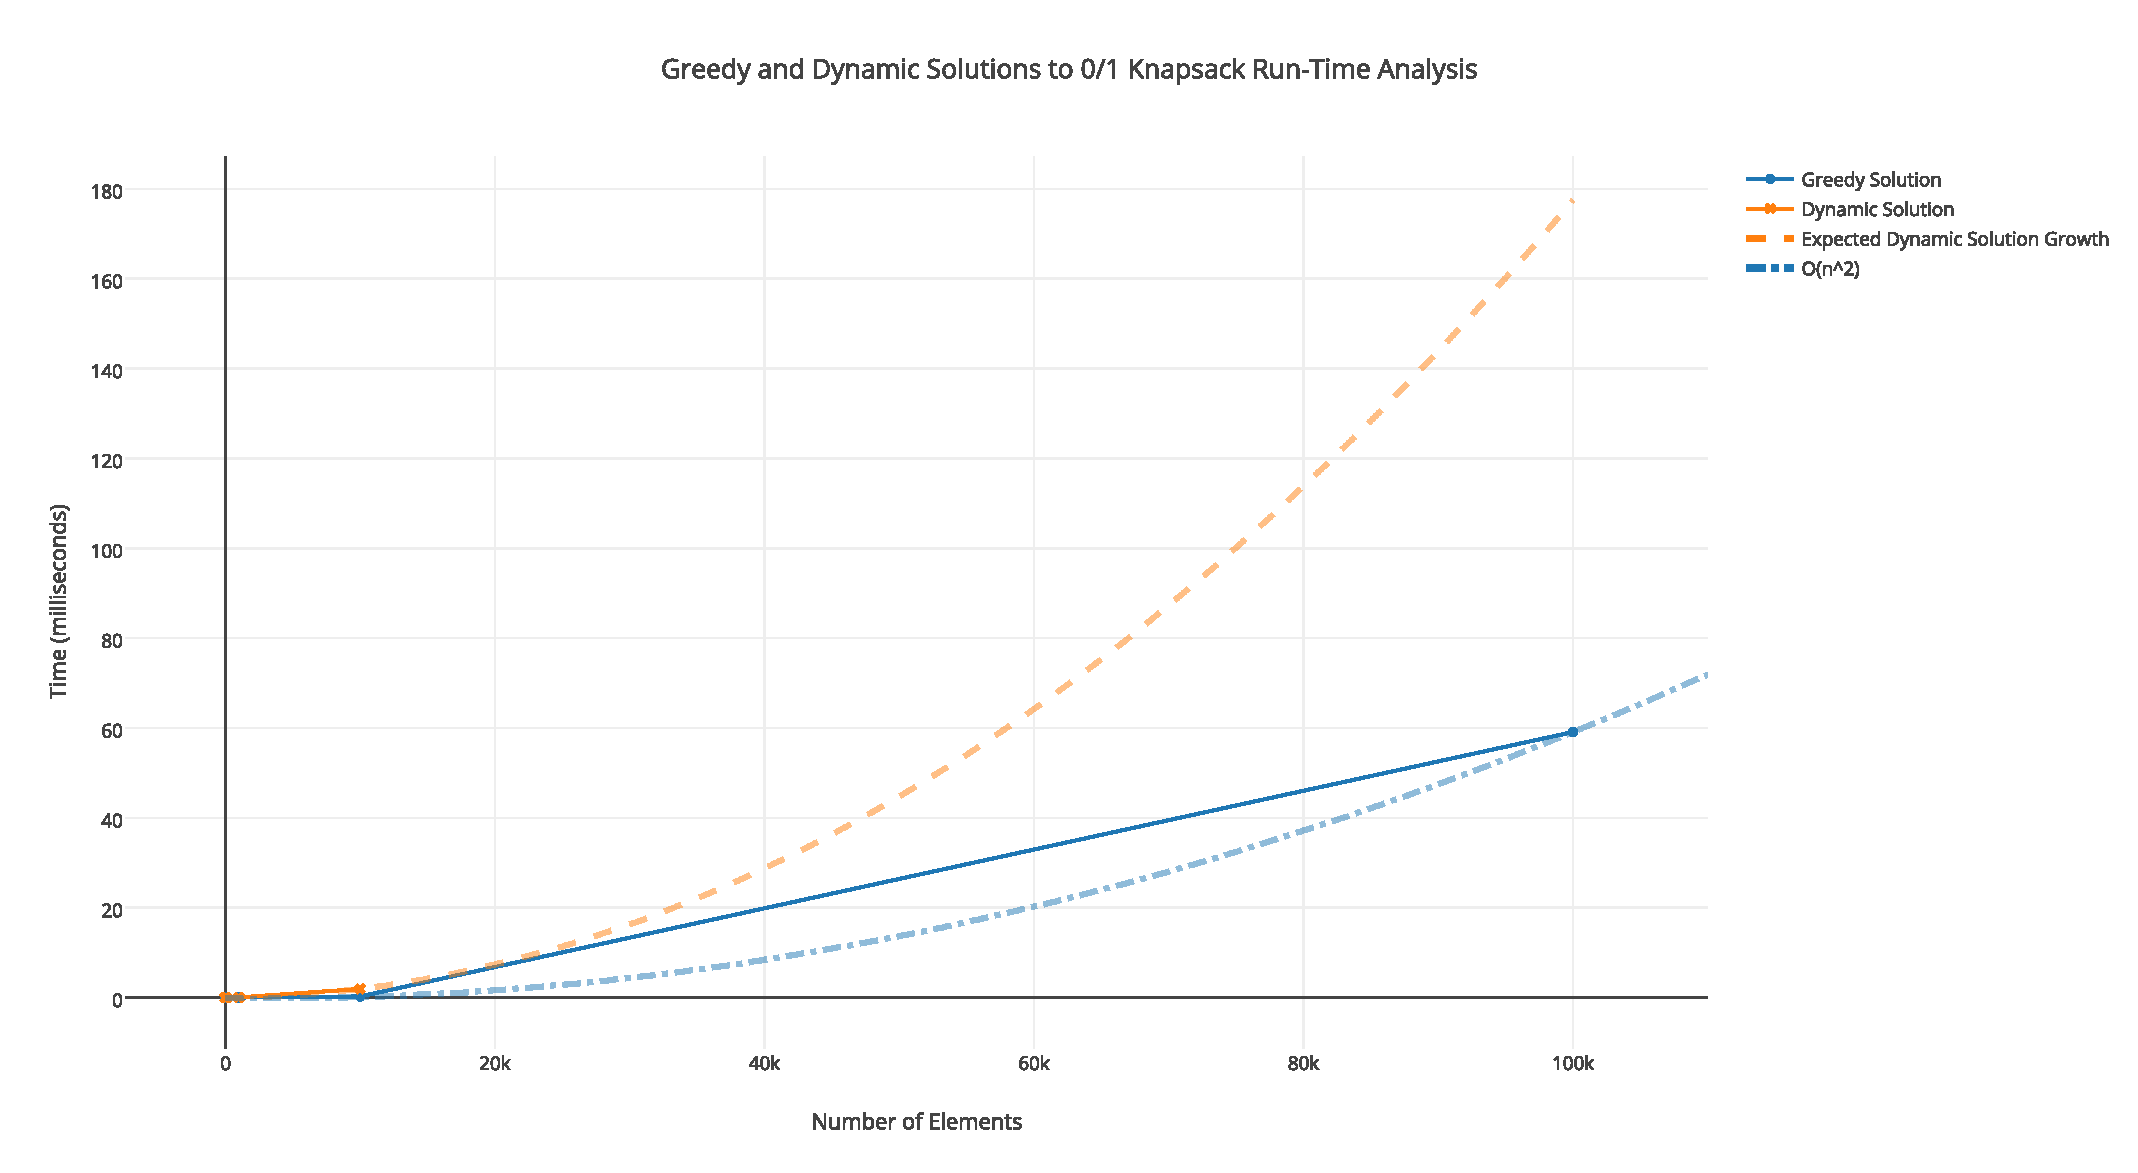
\includegraphics[scale=.55]{test-results.pdf}
\end{center}
\captionof{figure}{Java Implementation of Greedy and Dynamic Solutions to 0/1 Knapsack Run-Time Analysis}
\label{fig:runtime}
\end{figure}

%% END EXPERIMENTAL ANALYSIS

%% BEGIN CONCLUSION
\section{Conclusion}
%%TODO: write this

%% END CONCLUSION

\newpage

%% BEGIN REFERNCES
\section*{References}

%% \nocite{*}
%% \bibliographystyle{IEEEtran}
%% \bibliography{bib}

%% END REFERENCES

\newpage

%% BEGIN APPENDIX
\section*{Appendix}
\lstinputlisting[caption=Driver,
label={Driver.java},
breaklines=true,
]{Code/Driver.java}
\lstinputlisting[caption=Knapsack,
label={Knapsack.java},
breaklines=true,
]{Code/Knapsack.java}
\lstinputlisting[caption=Sort,
label={Sort.java},
breaklines=true,
]{Code/Sort.java}

The class Stopwatch has been altered from its original form.
\newline
\lstinputlisting[caption=Stopwatch,
label={Stopwatch.java},
breaklines=true,
]{Code/Stopwatch.java}
\lstinputlisting[caption=Debug,
label={Debug.java},
breaklines=true,
]{Code/Debug.java}
\lstinputlisting[caption=DummyData,
label={DummyData.java},
breaklines=true,
]{Code/DummyData.java}
%% END APPENDIX

%% END DOCUMENT
\end{document}
